%* 
%* ------------------------------------------------------------------
%* AN01_TheLayout.tex - Application Note 01: The Layout
%* Created by Robert Heller on Sun Sep 16 11:35:43 2012
%* ------------------------------------------------------------------
%* Modification History: $Log$
%* Modification History: Revision 1.1  2002/07/28 14:03:50  heller
%* Modification History: Add it copyright notice headers
%* Modification History:
%* ------------------------------------------------------------------
%* Contents:
%* ------------------------------------------------------------------
%*  
%*     Model RR System, Version 2
%*     Copyright (C) 1994,1995,2002-2012  Robert Heller D/B/A Deepwoods Software
%* 			51 Locke Hill Road
%* 			Wendell, MA 01379-9728
%* 
%*     This program is free software; you can redistribute it and/or modify
%*     it under the terms of the GNU General Public License as published by
%*     the Free Software Foundation; either version 2 of the License, or
%*     (at your option) any later version.
%* 
%*     This program is distributed in the hope that it will be useful,
%*     but WITHOUT ANY WARRANTY; without even the implied warranty of
%*     MERCHANTABILITY or FITNESS FOR A PARTICULAR PURPOSE.  See the
%*     GNU General Public License for more details.
%* 
%*     You should have received a copy of the GNU General Public License
%*     along with this program; if not, write to the Free Software
%*     Foundation, Inc., 675 Mass Ave, Cambridge, MA 02139, USA.
%* 
%*  
%* 

\chapter{The Layout}
\label{chapt:TheLayout}
\typeout{$Id$}

\begin{figure}[hbpt] 
\begin{centering}
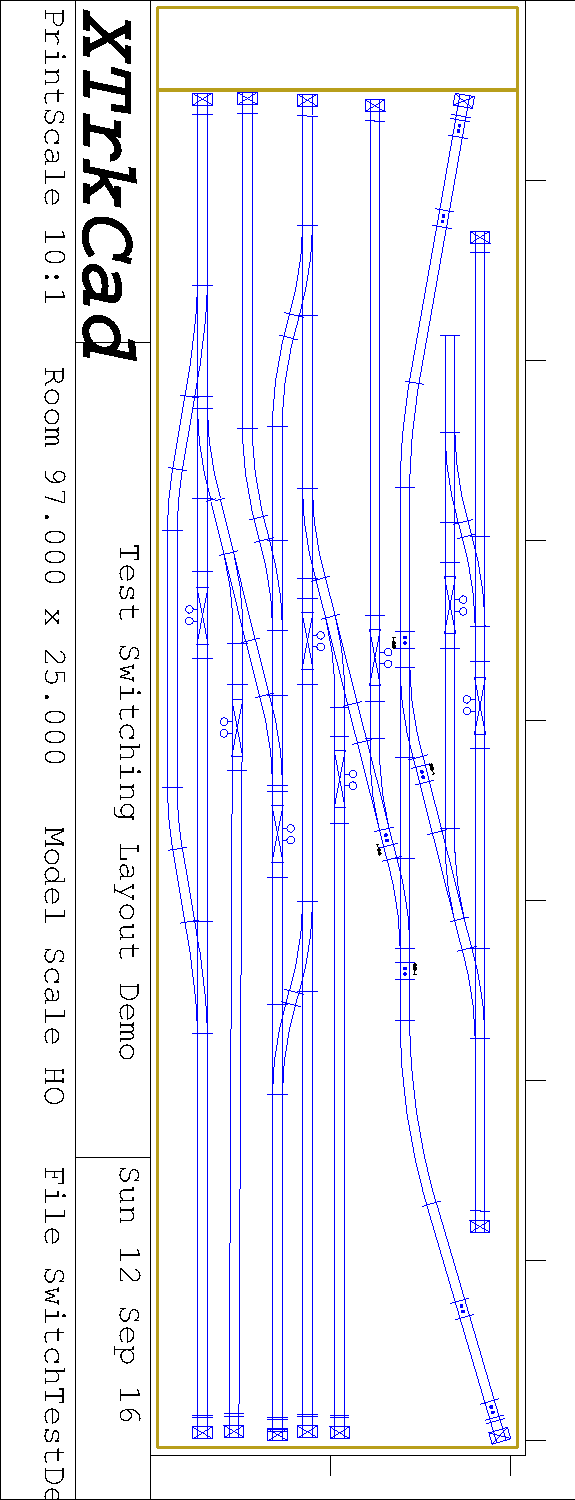
\includegraphics[angle=90,width=5in]{SwitchTestDemo.pdf}
\caption{Switch Test Demo Layout} 
\label{fig:TheLayout:SwitchTestDemo}
\end{centering} 
\end{figure}
The complete layout is shown in
Figure~\ref{fig:TheLayout:SwitchTestDemo}. This is a back and forth
switching yard layout, with a ``Main Line'' going through the middle of
the yard.  The yard ladder goes up the middle of the layout and
consists of a series of turnouts facing in different directions. There
are three places where a run around move can be made and almost all of
the tracks have a electro-magnetic uncompling ramp.  The turnouts
connecting the ``Main Line'' to the yard tracks are protected with
signals and these turnouts are under CTC control\footnote{These
turnouts require dispatcher (the computer) authority before they can be
thrown and the switch ``crew'' needs dispatcher authority before
entering onto the ``Main Line'' and shown by the signal aspects of the
interlocking signals.}.  The rest of the turnouts are in ``yard''
territory and are under local control and will be thrown by the switch
``crew''\footnote{They will be directly controled by buttons on the
Rail Driver.}. The sections that follow hightlight some of
the main features of this layout.

\section{Main line interlocking plant}

\begin{figure}[hbpt]
\begin{centering}
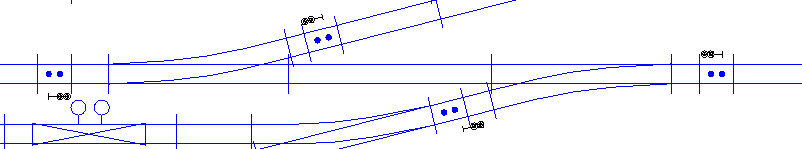
\includegraphics[width=5in]{SwitchTestDemo-MainInterlocking.png}
\caption{Main line interlocking plant}
\label{fig:TheLayout:SwitchTestDemo-MainInterlocking}
\end{centering}
\end{figure}
The main line interlocking plant, shown in
Figure~\ref{fig:TheLayout:SwitchTestDemo-MainInterlocking}, consists of
two opposed point turnouts and four two head (two over two) signals.
There are IR sensors at each aproach\footnote{Located at each of the
four signals.}.  The dispatcher, implemented as part of the software
program running on the computer, controls these two turnouts and the
signals that guard their aproaches.  Because of the regularly scheduled
commuter train, there are only limited windows when a switch job can
cross over the main line.  We will be using four Azatrak SR4-U units to
operate the signals, two Azatrak MRD2-U units to sense the presense of
trains at the aproaches to the interlocking plant, and an Azatrak SL2-U
to operate the turnouts.

\section{Commuter train stations at the ends of the main line.}

\begin{figure}[hbpt]
\begin{centering}
\mbox{\subfigure[Downtown station (west)]{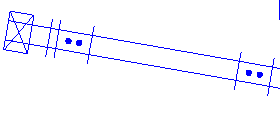
\includegraphics[width=2in]{SwitchTestDemo-DowntownStation.png}}\quad
      \subfigure[Suburbia Station (east)]{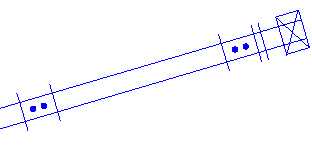
\includegraphics[width=2in]{SwitchTestDemo-SuburbiaStation.png}}}
\caption{Commuter train stations}
\label{fig:TheLayout:SwitchTestDemo-CommuterStations}
\end{centering}
\end{figure}
At each end of the main line is a commuter train station, as shown in
Figure~\ref{fig:TheLayout:SwitchTestDemo-CommuterStations}. We will use an
Azatrak MRD2-U unit for each station to detect when the commuter train
aproaches, arrives at, and leaves the station.  When the commuter train
aproaches, we will reduce its speed, when it arrives we will stop it and
reverse its direction (changing the headlights, marker lights and
rooftop flashers), and when it leaves the station we will increase its
speed to its full operating speed.


\section{Magnetic Uncoupling ramps}

\begin{figure}[hbpt]
\begin{centering}
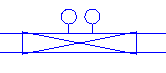
\includegraphics{SwitchTestDemo-UncouplingRamp.png}
\caption{Magnetic Uncoupling ramp}
\label{fig:TheLayout:SwitchTestDemo-UncouplingRamp}
\end{centering}
\end{figure}
There are eight Magnetic Uncoupling ramps, one of which is shown in
Figure~\ref{fig:TheLayout:SwitchTestDemo-UncouplingRamp}.  The coils of
these ramps will be activated using a NPN Darlington transistor circuit
\footnote{Using a TIP120 transistor.} controlled by one output of a
SR4-U device. We will build 2 circuit boards that hold 4 transistor switch
circuits each and use 2 SR4-Us to control these transistor switch
circuits, thus handling all 8 of the uncoupling ramps.

